\documentclass[12pt,a4paper]{article}
\usepackage[utf8]{inputenc}
\usepackage[spanish]{babel}
\usepackage{hyperref}
\usepackage{graphicx}

\title{Documentaci\'on del proyecto de \emph{Organizaci\'on de Computadoras} - \emph{Ta-Te-Ti}}
\author{Nicol\'as Dato y Nicol\'as Medina}
\date{03/11/2019}
\begin{document}

\maketitle

\newpage
\tableofcontents
\newpage

\section{Definiciones y especificaci\'on de requerimientos}

\subsection{Definici\'on general del proyecto de software}
	Este proyecto se basa en la creaci\'on del famoso juego \emph{Ta-Te-Ti}, el cual cuenta con 3 modos de juego, jugador vs jugador, jugador vs computadora y computadora vs computadora.

	El modo jugador vs jugador consiste simplemente en turnos donde cada jugador realizar\'a una jugada y se notificar\'a si esta se realiz\'o exitosamente, en caso de que no fuera as\'i (como intentar ubicar una ficha en una parte del tablero en el cual ya hab\'ia una) se pedir\'a realizar la jugada nuevamente. Las jugadas se ejecutar\'an decidiendo la posici\'on en la grilla, es decir, decidiendo el lugar mediante coordenadas $x$ e $y$ comenzando a contar desde $0$.

	Si se desea ejecutar uno de los dos modos donde participa la computadora, cuando sea su turno se ejecutar\'a el algoritmo de {\bf b\'usqueda adversaria MIN-MAX} donde se buscar\'a la mejor jugar\'a, dadas las caracter\'isticas del \emph{Ta-Te-Ti} esto significa que la computadora nunca pierde, s\'olo gana o empata.

    Cualquier persona que sepa las reglas del juego puede ser capaz de jugar, lo \'unico que tendr\'a que hacer es indicar $x$ e $y$ para colocar la ficha en la posici\'on que se quiera.

\subsection{Especificaci\'on de requerimientos del proyecto}
    La implementaci\'on del proyecto se ha realizado en el lenguaje C, el modo de visualizaci\'on del men\'u y tablero se ha realizado en la consola. Se ha implementado los {\itshape TDA LISTA} y {\itshape TDA ARBOL} los cuales se encontrara en una librer\'ia din\'amica denominada {\bf libliar} y esta se utilizara para el algoritmo de {\bf b\'usqueda adversaria MIN-MAX} el cual es implementado en un {\itshape TDA IA} . Tambi\'en se hizo uso de un {\itshape TDA PARTIDA} para el manejo del tablero, turnos, etc. Por ultimo, el programa principal se encargara de de manejar tanto el {\itshape TDA PARTIDA} como el {\itshape TDA IA} e ir\'a mostrando el estado actual del tablero.

    El usuario al iniciar el programa tendr\'a la opci\'on de iniciar una nueva partida o de salir del sistema, en caso de iniciar una nueva partida tendr\'a que elejir en qu\'e modo es el que desea jugar y luego decidir los turnos, tambi\'en se pedir\'a ingresar el nombre de los jugadores.

    El proyecto es un desarrollo original cumpliendo las pautas de implementacion dada por la c\'atedra de la materia {\itshape organizaci\'on de computadoras}, a\'un as\'i dado el desarrollo de clases y de estructura de datos aprendido en materias anteriores los {\itshape TDA} implementados en el lenguaje C pueden ser reutilizados en proyectos/desarrollos posteriores.

\subsection{Especificaci\'on de los procedimientos}

\subsubsection{Procedimientos de desarrollo}
    Como se dijo anteriormente, la implementaci\'on se realiz\'o en el lenguaje C y se ha usado como IDE y compilador de dicho lenguaje el dado por la c\'atedra llamado {\bf Code::Blocks y MinGW}. Se han usado varias librer\'ias de este lenguaje, las primeras dos son {\itshape stdlib.h} y {\itshape stdio.h} las cuales son las librer\'ias primordiales para el manejo de memoria y de I/O. Una de las otras librerias utilizadas fue {\itshape time.h} utilizada en el caso de que el usuario decida que empieza un jugador aleatorio. Otra librer\'ia utilizada fue la de {\itshape string.h} usada para copiar cadena de caracteres de una manera m\'as sencilla.

    Para abarcar este proyecto se decidi\'o primero la implementaci\'on del {\itshape TDA LISTA} para luego poder implementar el {\itshape TDA ARBOL} y as\'i estar en condiciones de encarar el algoritmo de {\bf b\'usqueda adversaria MIN-MAX}. Aun as\'i primero decidimos completar el {\itshape TDA PARTIDA} antes de desarrollar {\itshape TDA IA}.

    Una vez con todos los {\itshape TDA} completados se pas\'o a la implementaci\'on del programa principal, donde se implementa un menu facilitando la experiencia del usuario.

    Ya con todo finalizado se implement\' la librer\'ia {\bf libliar} con los {\itshape TDA LISTA} y {\itshape TDA ARBOL}.

\subsubsection{Procedimientos de compilaci\'on y ejecuci\'on}
    Para el uso del mismo, el usuario, el cual es as\'i mismo un desarrollador, contar\'a con el archivo comprimido {\bf .zip} conteniendo todos los archivos .cpb, .h y .c para la compilac\'on y ejecuci\'on del programa.
		
		Dado que se genera una librer\'ia (\emph{libliar}), se requiere abrir 2 proyectos con \emph{Code::Blocks}, tp1.cbp y libliar.cbp. En las propiedades del proyecto tp1 se puede configurar que tp1 tiene de dependencia el proyecto libliar\footnote{Lamentablemente no se logr\'o hacer que esta configuraci\'on quede guardada para que al abrir el proyecto ya est\'e la dependencia agregada}, para que al compilar tp1 tambi\'en se compile libliar.
		
		Para compilar el proyecto, primero que hay compilar libliar, que va a generar los archivos \emph{bin\textbackslash Debug\textbackslash libliar.a} y \emph{bin\textbackslash Debug\textbackslash libliar.dll}.
		
		Con libliar compilado, se puede compilar el proyecto tp1, el cual va a linkearse con \emph{bin\textbackslash Debug\textbackslash libliar.a}\footnote{Con \emph{Code::Blocks} no se logr\'o utilizar el archivo .dll, la \'unica opci\'on que hab\'ia era linkear contra el archivo .a, de todas formas el archivo .dll se genera y est\'a disponible.}
		
		Una vez compilado el proyecto tp1, en \emph{bin\textbackslash Debug\textbackslash} se genera el archivo \emph{tp1.exe} para ser ejecutado.

\section{Arquitectura del sistema}

\subsection{Descripci\'on jer\'arquica}
    La arquitectura del sistema cuenta con un programa principal llamado {\bf main} el cual se encarga de usar el {\itshape TDA PARTIDA} para la creaci\'on y administraci\'on de la misma, tambi\'en en el {\bf main} usar\'a el {\itshape TDA IA} en casos de ser necesario, es decir, si el usuario desea iniciar uno de los dos modos donde juega la computadora.

    El {\itshape TDA IA} utiliza el algoritmo de {\bf b\'usqueda adversaria MIN-MAX}, tambi\'en usar\'a al {\itshape TDA PARTIDA} y {\itshape TDA ARBOL}.

    Por \'ultimo el {\itshape TDA ARBOL} usar\'a al {\itshape TDA LISTA} para guardar una lista de sus hijos.

\subsection{Diagrama de m\'odulos}
\begin{figure}[h!tbp]
	\centering
		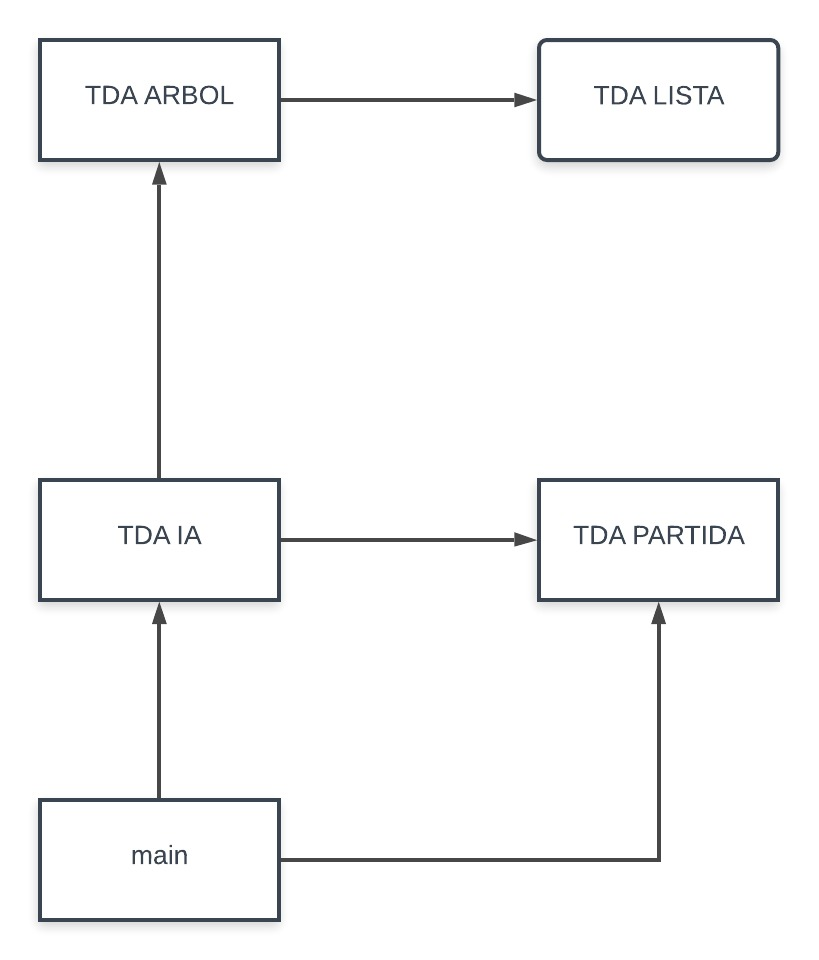
\includegraphics[width=1.00\textwidth]{diagrama.jpg}
	\label{fig:diagrama}
\end{figure}

\newpage

\subsection{Descripci\'on general de los m\'odulos}
\subsubsection{Descripci\'on general y prop\'osito}
\begin{itemize}
    \item {\bf TDA LISTA}: Implementa nodos enlazados los cuales apuntan al siguiente nodo y almacenan un elemento gen\'erico. La posici\'on es indirecta y tiene un nodo centinela.
	\item {\bf TDA ARBOL}: Implementa \emph{tnodos} los cuales apuntan a su \emph{tnodo} padre (en caso de no ser la raiz), almacenan un elemento gen\'erico y una lista de hijos.
    \item {\bf TDA PARTIDA}: Implementa una partida con informaci\'on actual de la misma. La partida guarda tanto los nombres de los jugadores, el turno del jugador al que le toca jugar, el estado actual de la partida (si alguien gan\'o, etc) y el modo de la partida que se est\'a jugando. El tablero apunta a una grilla de 3x3 la cual guarda el estado del mismo teniendo en cada posici\'on los valores $0$, $1$ o $2$ para el caso de una casilla vac\'ia, una ficha del jugador 1 o una ficha del jugador 2, respectivamente.
    \item {\bf TDA IA}: Implementa un estado y una b\'usqueda adversaria. El estado guarda una grilla de 3x3 con la que fue llamada y la utilidad el cual representa el resultado de la grilla (si se sigue jugando, alguien gan\'o, etc). Busqueda adversaria apunta a un \'arbol y a dos enteros, el jugador max y el jugador min. Con esta informaci\'on el algoritmo buscar\'a la mejor jugada que puede realizar el jugador.
    \item {\bf main}: Implementa un men\'u en la consola el cual administra el {\itshape TDA PARTIDA} y el {\itshape TDA IA} en caso de ser necesario.
\end{itemize}

\subsubsection{Responsabilidad y restricciones}
\begin{itemize}
    \item {\bf TDA LISTA}: La lista espera que cuando se le ingrese un elemento ya tenga un espacio en memoria asignado. La lista, al eliminar o destruir espera una funci\'on con la cual eleminar\'a al elemento y liberar\'a el espacio asignado a memoria del mismo. Al insertar un elemento lo asignar\'a como siguiente a la posici\'on recibida.
    \item {\bf TDA ARBOL}: El arbol espera despu\'es de ser creado que se le asigne una ra\'iz como primer elemento, y en caso de que se le intente asignar un nodo que no sea ra\'iz se informar\'a de un error. Tambi\'en cuando se desee insertar un elemento se le tiene que asignar un espacio en memoria al mismo previamente. Al eliminar o destruir, de igual manera que la lista se espera que se le pase una funci\'on por par\'ametro la cual se encargara del eliminar y borrar de la memoria al elemento. Al insertar un elemento se esperan dos tnodos, el primero de ellos debe ser el padre al cual se le desea agregar un hijo y el segundo es el hermano derecho al nodo a insertar, en caso de que el segundo nodo sea NULL el elemento se asigna como el \'ultimo hijo del tnodo padre.
    \item {\bf TDA PARTIDA}: La partida lo que espera como modo y turno son enteros, asociados a constantes ya definidas en el TDA, en el caso del nombre se espera como m\'aximo 49 caracteres. Si dado al caso se intenta hacer un movimiento en una casilla ya ocupada, retornar\'a un error.
    \item {\bf TDA IA}: La ia al momento de crear la b\'usqueda adversaria lo que espera es que se le haya pasado correctamente la partida en su estado actual, para as\'i poder empezar con el algoritmo. En el caso de resultado esperado lo que espera la ia es que el resultado buscado siempre sea el mejor, es decir, gana max, ya que la ia nunca pierde, s\'olo gana o empata. Tambi\'en espera dos punteros a enteros los cuales va a modificar con la posici\'on en la cual esta la mejor jugada posible.
    \item {\bf main}: El main tiene limitaciones al ejecutarse por consola, las cuales son que los nombres de los jugadores no podr\'an exceder los 49 caracteres, y la segunda es que espera que cada vez que da una opci\'on a elegir espera un n\'umero entero.
\end{itemize}

\subsubsection{Dependencias}
\begin{itemize}
    \item {\bf TDA LISTA}: Este TDA no requiere de ningun paquete externo o librer\'ia ademas de las librerias esenciales proporcionadas por C.
    \item {\bf TDA ARBOL}: Este TDA de la librer\'ia del {\itshape TDA LISTA} ya mencionado.
    \item {\bf TDA PARTIDA}: Este TDA adem\'as de las librer\'ias esenciales de C requiere de las  librer\'ias {\itshape time.h} y {\itshape string.h}.
    \item {\bf TDA IA}: Este TDA requiere de los {\itshape TDA PARTIDA} y {\itshape TDA ARBOL} ya mencionados.
    \item {\bf main}: El main solo requiere del {\itshape TDA IA} debido a que este ya tiene contenido todo el resto de los TDA y librer\'ias.
\end{itemize}

\subsubsection{Implementaci\'on}
\begin{itemize}
    \item {\bf TDA LISTA}: Este TDA se encuentra implementado en la librer\'ia din\'amina llamada {\bf libliar}.
    \item {\bf TDA ARBOL}: Este TDA se encuentra implementado en la librer\'ia din\'amica llamada {\bf libliar}.
    \item {\bf TDA PARTIDA}: Este TDA se encontrar\'a definido en un .h denominado {\itshape partida.h} e implementado en un .c llamado {\itshape partida.c}. Estos archivos se encontraran en el {\bf .zip}.
    \item {\bf TDA IA}: Este TDA al igual que el anterior se encuentra definido en {\itshape ia.h} e implementado en {\itshape ia.c}. Estos archivos se encontrar\'an en el {\bf .zip}.
    \item {\bf main}: Este se encuentra implementado en {\itshape main.c}. Este archivo se encontrar\'a en el {\bf .zip}.
    \item {\bf libliar}: Librer\'ia din\'amica con los {\itshape TDA LISTA} y {\itshape TDA ARBOL}, se encontrar\'a en el {\bf .zip}.
\end{itemize}

\subsection{Dependencias externas}
\begin{itemize}
    \item {\bf stdio.h}: Es la librer\'ia que contiene las definiciones de las macros, las constantes, las declaraciones de funciones de la biblioteca est\'andar del lenguaje de programaci\'on C para hacer operaciones de entrada y salida, as\'i como la definici\'on de tipos necesarias para dichas operaciones.
    \item {\bf stdlib.h}: Es la librer\'a cabecera de la biblioteca est\'andar de prop\'osito general del lenguaje de programaci\'on C. Contiene los prototipos de funciones de C para gesti\'on de memoria din\'amica, control de procesos y otros.
    \item {\bf time.h}: Es la librer\'ia relacionada con formato de hora y fecha, es un archivo de cabecera de la biblioteca est\'andar del lenguaje de programaci\'on C que contiene funciones para manipular y formatear la fecha y hora del sistema.
    \item {\bf string.h}: Es una librer\'ia de la biblioteca est\'andar del lenguaje de programaci\'on C que contiene la definici\'on de macros, constantes, funciones y tipos y algunas operaciones de manipulaci\'on de memoria relacionadas a cadena de caracteres.
\end{itemize}

\section{Descripci\'on de procesos y servicios ofrecidos por el sistema}
\subsection{Invocaci\'on del programa}
Para ejecutar el programa s\'olo basta con ejecutar \emph{tp1.exe}. No espera ning\'un par\'ametro.

\subsection{TDA LISTA}
\subsubsection{Creaci\'on de la lista}
La lista se crea en la funci\'on \emph{crear\_lista(tLista *l)}, la cual crear\'a en $l$ una nueva estructura y la inicializar\'a con los valores de una lista vac\'ia, es decir una lista con el elemento centinela pero sin m\'as elementos.

\subsubsection{Insertar elemento}
Para insertar elemento est\'a la funci\'on \emph{void l\_insertar(tLista l, tPosicion p, tElemento e)}, esta funci\'on crea una nueva celda y la inserta en la posici\'on indicada. Dado que se trabaja con posici\'on indirecta, para insertar se tiene que agregar la celda nueva en \emph{p.siguiente} para que al recuperar el elemento en la posici\'on $p$ se obtenga el elemento insertado. El anterior elemento en $p$ pasar\'a a ser el siguiente del nodo insertado.

\subsubsection{Eliminar elemento y destrucci\'on de la lista}
Las funciones \emph{void l\_destruir(tLista * l, void (*fEliminar)(tElemento))} y \emph{void l\_eliminar(tLista l, tPosicion p, void (*fEliminar)(tElemento))} destruyen la lista y eliminan un nodo, respectivamente. Al eliminar un nodo lo que se hace es eliminar \emph{p.siguiente} dado que se trabaja con posici\'on indirecta, y eliminando el elemento de la celda con $fEliminar$. En el caso de destruir la lista el procedimiento es similar, eliminando todos los elementos de la lista para luego eliminar la lista en s\'i. Los nodos y la lista se eliminan con \emph{free()}.

\subsubsection{Obtener posiciones de los nodos y la longitud de la lista}
Para obtener la primera posici\'on, la anterior y siguiente de una posic\'on, la \'ultima posici\'on y el fin de la lista se tiene las funciones \emph{tPosicion l\_primera(tLista l)}, \emph{tPosicion l\_anterior(tLista l, tPosicion p)}, \emph{tPosicion l\_siguiente(tLista l, tPosicion p)}, \emph{tPosicion l\_ultima(tLista l)}, \emph{tPosicion l\_fin(tLista l)}. Teniendo en cuenta que se trabaja con posici\'on indirecta estas funciones resultan triviales. 

Para recuperar el elemento de una posici\'on se utiliza la funci\'on \emph{tElemento l\_recuperar(tLista l, tPosicion p)}

La longitud de la lista se obtiene \emph{int l\_longitud(tLista l)}, una funci\'on recursiva que tiene de caso base la lista vac\'ia (longitud $0$) y sino suma $1$ por cada elemento recursivamente hasta llegar al caso base.

\subsection{TDA ARBOL}
\subsubsection{Creaci\'on del \'arbol y su ra\'iz}
El \'arbol se crea con la funci\'on \emph{void crear\_arbol(tArbol * a)}, que va a crear un \'arbol sin ra\'iz. Para ingresarle la ra\'iz hay que llamar a \emph{void crear\_raiz(tArbol a, tElemento e)}.

El \'arbol estar\'a representado como nodos, donde cada nodo tiene un puntero a su padre y tiene una lista de hijos.

\subsubsection{Ingresar elemento}
Para ingresar elementos al \'arbol, existe la funci\'on \emph{tNodo a\_insertar(tArbol a, tNodo np, tNodo nh, tElemento e)}, la cual ingresa el elemento $e$ como hijo de $np$ a la izquierda de $nh$, si $nh$ es $NULL$ entonces se ingresa como \'ultimo hijo de $np$.

Al ingresar un elemento se crea un nodo nuevo y con una lista vac\'ia de hijos, en caso de que $nh$ sea $NULL$ se ingresa el nuevo nodo al final de la lista de hijos de $np$; pero si $nh$ no es $NULL$ entonces primero se busca a $nh$ entre los hijos de $np$ para poder ingresar el nuevo nodo antes de $nh$.

\subsubsection{Eliminar elemento y destrucci\'on del \'arbol}
Las funciones \emph{void a\_eliminar(tArbol a, tNodo n, void (*fEliminar)(tElemento))} y \emph{void a\_destruir(tArbol * a, void (*fEliminar)(tElemento))} eliminan un elemento y destruyen el \'arbol respectivamente.

Para eliminar un elemento, hay 3 casos v\'alidos: que sea la ra\'iz sin hijos, que sea la ra\'iz con s\'olo un hijo, que no sea la ra\'iz; en todos los casos se destruye la lista de hijos y se elimina el elemento de la con $fEliminar$.

En el caso de que sea una ra\'iz sin hijos, s\'olo se quita la ra\'iz del \'arbol. Cuando sea la ra\'iz con un \'unico hijo, ese elemento pasa a ser la nueva ra\'iz.

Si el elemento a eliminar es un nodo que no es ra\'iz, entonces todos los hijos del nodo pasan a estar como hijos del padre, en el mismo orden y en el lugar donde estaba el nodo. Para realizar esta operaci\'on se tuvo que usar una funci\'on \emph{no\_eliminar()} que no hace nada y pasar esa funci\'on a \emph{l\_eliminar()}. Esto se debe a que se necesita quitar los elementos del nodo sin eliminarlos para poder ingresarlos como hijos del padre, pero la interface del \emph{TDA LISTA} no tiene una forma de quitar el elemento sin que se llame a una funci\'on de eliminado, entonces con \emph{no\_eliminar()} el nodo es eliminado de la lista pero sin destruir al elemento y se puede as\'i recuperar un elemento de la lista, eliminarlo de la lista sin que se elimine el elemento en si, y luego colocar el elemento recuperado en otra lista.

Para la destrucci\'on de todo el \'arbol, se utiliza una funci\'on auxiliar \emph{n\_eliminar(tNodo n, void (*fEliminar)(tElemento))} que va a eliminar al elemento del nodo $n$ y luego recursivamente va a eliminar los nodos hijos de $n$ para luego destruir la lista.

\subsubsection{Obtener elementos}
Para operar con el \'arbol y obtener elementos, est\'an las funciones \emph{tNodo a\_raiz(tArbol a)}, \emph{tLista a\_hijos(tArbol a, tNodo n)} y \emph{tElemento a\_recuperar(tArbol a, tNodo n)} que van a devolver el nodo ra\'iz, una lista de \emph{tNodo} hijos de un nodo, y obtener el elemento del nodo respectivamente. Son funciones triviales.

\subsubsection{Sub\'arbol}
Se puede obtener un sub\'arbol utilizando \emph{void a\_sub\_arbol(tArbol a, tNodo n, tArbol * sa)}. Esa funci\'on va a crear un nuevo \'arbol en $sa$ donde $n$ es ra\'iz con todos sus hijos, y en el \'arbol original $a$ se quita a $n$ y sus hijos.

Para realizar esto se busca al nodo $n$ en la lista de hijos de su padre, y se lo quita sin destruir al elemento (utilizando la func\'on \emph{no\_eliminar()} tal como se hac\'ia en \emph{a\_eliminar()}).

\subsection{TDA PARTIDA}
\subsubsection{Crear partida nueva y finalizarla}
Para crear una nueva partida hay que llamar a la funci\'on \emph{void nueva\_partida(tPartida * p, int modo\_partida, int comienza, char * j1\_nombre, char * j2\_nombre)}, y se va a inicializar las estructuras con el modo de la partida, qui\'en comienza, los nombres de los jugadores y un tablero sin fichas colocadas (todas las posiciones en $0$). Si el jugador que comienza fuese aleatorio, se pide un n\'umero pseudo-aleatorio con \emph{rand()}, si el resultado es par comienza el jugador 1, si no comienza el jugador 2.

Para finalizar la partida se utiliza la funci\'on \emph{finalizar\_partida(tPartida * p)}, la cual va a eliminar la memoria utilizada para la partida.

\subsubsection{Realizar movimientos}
Se pueden realizar movimientos en el tablero con la fuci\'on \emph{int nuevo\_movimiento(tPartida p, int mov\_x, int mov\_y)}, se va a corroborar que la posici\'on se encuentre vac\'ia y va a realizar la jugada colocando un $1$ para el jugador 1 y un $2$ para el jugador 2. Luego revisa el tablero para saber si con la jugada realizada hay un ganador, o es empate, o si se puede seguir jugando.

\subsection{TDA IA}
\subsubsection{Creaci\'on y destrucci\'on de b\'usqueda adversaria}
La b\'usqueda adversaria, utilizada para saber el mejor movimiento a realizar, se crea con \\\emph{void crear\_busqueda\_adversaria(tBusquedaAdversaria * b, tPartida p)}. Se va a crear un \'arbol donde se va a ejecutar el algoritmo \emph{Min-Max}, siendo la ra\'iz del \'arbol el tablero actual y siempre arrancando a jugar como \emph{Max} para maximizar la jugada. El \'arbol se crea de tal forma de que en cada nivel se vaya alternando entre \emph{Min} y \emph{Max}, se llama recusrivamente con cada uno de los posibles movimientos a realizar y luego se buscar\'a la mejor jugada en el caso de ser \emph{Max} o la peor jugada en el caso de ser \emph{Min}. Tambi\'en se detendr\'a la b\'usqueda si se encuentra con una jugada ganadora o perdedora (seg\'un sea \emph{Max} o \emph{Min}) para no seguir procesando el \'arbol cuando no es necesario por que no podr\'a haber mejores resultados.

Para destruir la b\'usqueda adversaria hay que llamar a \\\emph{void destruir\_busqueda\_adversaria(tBusquedaAdversaria * b)} que va a destruir el \'arbol y liberar la memoria utilizada.

\subsubsection{Obtenci\'on del pr\'oximo movimiento}
Una vez creada la b\'usqueda adversaria, se utiliza \\\emph{void proximo\_movimiento(tBusquedaAdversaria b, int resultado\_esperado, int * x, int * y)} para obtener el mejor movimiento. Esta funci\'on va a revisar los hijos de la ra\'iz (es decir, las posibles jugadas que se tienen a partir del estado actual) y se va a quedar con la mejor jugada de todas, luego comparando el tablero actual con el tablero de la mejor jugada se obtiene la diferencia y se indican en $x$ e $y$ las coordenadas a jugar. Dada la forma en que se crea el \'arbol para el algoritmo \emph{Min-Max}, el valor de utilidad de la ra\'iz va a ser la utilidad de la mejor jugada de sus hijos (dado que la ra\'iz es siempre \emph{Max}), por lo que buscar la mejor jugada entre los hijos es buscar al hijo que tenga la misma utilidad que la ra\'iz.

\subsection{Main - programa principal}
El programa principal primero va a pedir toda la informaci\'on de la partida (jugadores, modo, etc.) y va a crear una nueva partida. Luego va a iterar mientras no haya ganadores ni empate y va a pedir las coordenadas de la ficha al jugador y va a realizar la jugada. En caso de que sea el turno de la m\'aquina va a crear la b\'usqueda adversaria del \emph{TDA IA}, va a buscar la mejor jugada y la va a realizar.

Una vez terminado el juego se pregunta al usuario si se quiere seguir jugando o si se quiere salir, pudiendo jugar nuevamente sin reiniciar el programa.

\section{Conclusiones}
Lo m\'as novedoso y que m\'as cost\'o entender fue el algoritmo de \emph{Min-Max}, entre otras cosas por algunas diferencias entre la el pseudoc\'odigo del algoritmo y la interface que hab\'ia que implementar. Pero lo pudimos resolver y parece estar funcionando adecuadamente.

El an\'alisis del tablero para saber si hay alg\'un ganador lo intentamos hacer s\'olo revisando la posici\'on jugada y sus alrededores (sin recorrer todo el tablero), pero luego de algunos intentos fallidos (andaba para algunos casos y para otros no), optamos por analizar todo el tablero para saber si hay alg\'un ganador o empate.

Al implementar el \emph{TDA ARBOL} nos encontramos con una limitaci\'on del \emph{TDA LISTA}, no se puede quitar un elemento de la lista sin eliminarlo. Nos hubiera gustado que la interfaz incluya una funci\'on que retorne el elemento y al mismo tiempo lo quite de la lista, de esa forma se pueden mover elementos de una lista a otra sin tener que eliminarlos y recrearlos. Pero para sortear este tema optamos por hacer una funci\'on que no hace nada y pasar esta funci\'on al momento de querer eliminar un elemento de la lista, as\'i podemos recuperar un elemento, eliminarlo de la lista sin que se elimine el elemento en si, y luego colocar el elemento en otra lista. Esto fue necesario al eliminar nodos y al crear un sub-\'arbol donde hay que operar con las listas y sus nodos y cambiarlos de lugar.

Si se ingresa el juego en modo \emph{Computadora-vs-Computadora} el resultado es un empate, que es lo esperado dado que en \emph{Ta-Te-Ti} si ambos jugadores juegan la mejor jugada es un empate. Notamos que la primer jugada de la computadora no es en el centro sino en una esquina, creemos que esto sucede por que con el tablero vac\'io no hay ninguna jugada que sea ganadora, la mejor jugada va a ser un empate, y entonces jugando tanto en el centro como en la esquina el resultado sea empate y por algo de la implementaci\'on o de la forma que se recorre/genera el \'arbol la m\'aquina se quede con la jugada de la esquina.

\end{document}
